\chapter{Grundlagen}
\label{chap:basics}

Bevor die Ziele der Migration von Flow zu TypeScript im nächsten Kapitel dargelegt werden, sollen zunächst die nötigen theoretischen Grundlagen dargestellt werden, um die Nachvollziehbarkeit der weiteren Ausführungen zu erleichtern. Dazu werden im Folgenden drei Konzepte aus der Theorie der Typensysteme erläutert.

\section{Konzepte und Begriffe der Typentheorie}

\subsection{Korrektheit von Typsystemen}
Ein wichtige Eigenschaft von Typsystemen ist deren logische \emph{Korrektheit}\footnote{engl. \textit{soundness}.}. Dieses Kriterium beschreibt, ob das System garantieren kann, dass ein Programm während dessen Ausführung tatsächlich keine Typfehler verursacht, sofern keine statischen Typverletzungen bestehen~\autocite{WRIGHT:1994}. In einem solchen System stimmt also der Typ eines zur Laufzeit ausgewerteten Ausdrucks stets mit dem statischen Typ überein~\autocite{DART:TYPE_SYSTEM}. Durch mathematische Formalisierung kann diese Eigenschaft bewiesen werden~\autocite[7]{CARDELLI:TYPE_SYSTEMS}. Das Gegenstück von Korrektheit ist \textit{Vollständigkeit}. Während ein korrektes System alle Fehler identifiziert, die zur Laufzeit auftreten können, findet ein vollständiges System nur diejenigen Fehler, die tatsächlich während der Ausführung eintreten würden~\autocite{FLOW:TYPES_AND_EXPRESSIONS}. Im ersten Fall werden unter Umständen Fehler entdeckt, die zur Laufzeit praktisch nicht vorkommen (falsch positiver Fehler), im zweiten Fall treten dagegen eventuell Laufzeitfehler auf, obwohl keine Typverletzung festgestellt wurde (falsch negativer Fehler). Im Idealfall ist ein Typsystem sowohl korrekt, als auch vollständig.

Das Typsystem mancher Programmiersprachen erfüllt diese Definition von Korrektheit nicht. So ist die Semantik bestimmter Operationen in C wie beispielsweise die Dereferenzierung des Nullzeigers in der Sprachspezikation undefiniert~\autocite[79]{ISO:C99}. Obwohl ein solches Programm durch den Compiler akzeptiert wird, also keine Typverletzungen aufweist, können hier Laufzeitfehler auftreten.

\subsection{Subtyping}

Die zwei in dieser Arbeit betrachteten Typsysteme Flow~\autocite{FLOW:PAPER} und TypeScript~\autocite{TYPESCRIPT:SPEC} setzen Subtyping ein~\autocites{FLOW:PAPER,BIERMAN:2014}. Weil dieses Konzept bedeutsam für das Verständnis der weiteren Ausführungen ist, soll dieses erklärt werden. Ein Typ kann als eine Menge von Werten betrachtet werden. Zum Beispiel umfasst der Typ \code{string} von JavaScript alle Zeichenketten, die durch die Sprachspezifikation möglich sind.
Subtyping stellt die Relation dar, die aussagt, ob ein Typ T Untertyp eines anderen Typen S ist~\autocite[27\psq]{CARDELLI:TYPE_SYSTEMS}. Hierfür muss das Kriterium der \emph{Subsumtion} erfüllt sein. Diese besteht, wenn die Menge, die S darstellt, jeden Wert von T beinhaltet. Folglich kann der Typ T überall dort eingesetzt werden, wo S erwartet wird (\textit{Liskovsches Substitutionsprinzip}). Bezogen auf das Beispiel bedeutet dies, dass der Typ der Zeichenkette \enquote{\textit{abc}} Untertyp von \code{string} ist, weil die Menge aller Werte von \code{string} auch dieses Wort enthält.

Zwei weitere Begriff in diesem Zusammenhang, die im weiteren Verlauf verwendet werden, sind \emph{Kovarianz} und \emph{Kontravarianz}. Dabei bedeutet Kovarianz eine Betrachtung \emph{in} Richtung der Subtyp-Hierarchie, Kontravarianz \emph{entgegen} dieser~\autocite{VARIANCE}. Im Fall von Kovarianz werden Subtypen aber keine Supertypen akzeptiert, bei Kontravarianz hingegen nur Supertypen, aber keine Subtypen~\autocite{FLOW:VARIANCE}.

\subsection{Nominale und strukturelle Typen}
Eine Möglichkeit Typsysteme zu klassifizieren, ist die Verwendung von \textit{nominalen} bzw. \textit{strukturellen} Typen. Da sich Flow und TypeScript in diesem Aspekt unterscheiden, soll auch diese Differenzierung dargelegt werden. Entscheidend ist hierbei die Fragestellung, ob unabhängige Typen durch das Typsystem als äquivalent angesehen werden oder nicht~\autocite[9]{CARDELLI:TYPE_SYSTEMS}. Bedeutsam ist auch, wann ein Typ als Untertyp eines anderen Typen betrachtet wird. Bei strukturellen Typen liegt ein Subtyp vor, wenn dessen Attribute eine Obermenge des Supertyps sind~\autocite{MALAYERI:2008}. Liegt hingegen ein nominaler Typ vor, so besteht eine solche Beziehung nur genau dann, wenn sie explizit, zum Beispiel durch das Schlüsselwort \code{extends}, deklariert wird. Die Typsysteme der meisten Programmiersprachen setzen sowohl nominale, als auch strukturelle Typen ein~\autocite[9]{CARDELLI:TYPE_SYSTEMS}. Anhand eines Beispiels in Pseudocode (Quelltext~\ref{code:type-equivalence}) soll diese Differenzierung verdeutlicht werden.

\begin{lstlisting}[
  label={code:type-equivalence},
  caption={Beispiel zur Differenzierung von nominalen und strukturellen Typen.}
]
class A { prop: string; }
class B { prop: string; }
function f(arg: A) {}
f(new B()); // << Typfehler?
\end{lstlisting}

In den ersten beiden Zeilen werden zunächst zwei Klassen \code{A} und \code{B} definiert. Weiterhin wird eine Funktion \code{f} angegeben, die einen Parameter vom Typ \code{A} erwartet. Bei Aufruf dieser Funktion mit einer Instanz der Klasse \code{B} sind nun zwei Fälle möglich: Entweder spezifiziert das System, dass Typen mit unterschiedlichen Namen stets inkompatibel sind, oder die Typen \code{A} und \code{B} werden als äquivalent betrachtet, da ihre Struktur übereinstimmt. Im ersten Fall würde in Zeile~4 eine Typverletzung auftreten, da der Typ des Ausdrucks \code{new B()} nicht \code{A}, sondern \code{B} ist. Läge hingegen eine strukturelle Typisierung vor, so würde das Programm akzeptiert werden, da der Aufbau der Klassen \code{A} und \code{B} identisch ist. Beide enthalten genau ein Attribut \code{prop} mit demselben Typ \code{string}.

\section{Statische Typsysteme für JavaScript}
\label{sec:static-typesystems-for-js}

% Im Folgenden sollen einige bestehende Ansätze betrachtet werden, die eine statische Typisierung in JavaScript ermöglichen. Die Idee, die ausgeführten Schwachstellen des dynamischen Typsystems der Sprache so auszugleichen, ist nicht neu~\autocite[2]{FLOW:PAPER}: Innerhalb der letzten Jahre sind verschiedene Ansätze entstanden, die sich dieser Problematik widmen.
% Ein Beispiel ist das 2009 erschienene Werkzeug \textit{Closure Compiler}~\autocite{CLOSURE:COMPILER}. Ziel dieses Transpilers ist es einerseits gängige Programmierfehler in JavaScript-Quelltexten mittels statischer Analyse aufzudecken, andererseits effizienteren Ausgabecode durch Anwendung verschiedener Optimierungen zu erzeugen~\autocite{CLOSURE:COMPILER}. Darüber hinaus ist es möglich Ausdrücke innerhalb des Quelltexts durch spezielle Annotationen in Kommentaren zu typisieren, sodass der Compiler daraufhin die Typkorrektheit statisch überprüfen kann~\autocite{CLOSURE:TYPES}. Zum Beispiel kann durch folgende Notation eine (schreibgeschützte) Konstante hergestellt werden:

% \begin{lstlisting}[numbers=none]
% /** @const */ var PI = 3.14;
% \end{lstlisting}

% Einen anderen Ansatz verfolgt die Programmiersprache \textit{Dart}~\autocite{DART:SPEC}. Dart bietet ein gemäß obiger Definition korrektes, statisches Typsystem, welches neben konventionellen Typdeklarationen auch Typinferenz unterstützt~\autocite{DART:TYPE_SYSTEM}. Anstatt JavaScript durch Typannotationen in Kommentaren zu erweitern, wird hier also auf eine andere Programmiersprache mit statischer Typisierung zurückgegriffen, die in äquivalenten JavaScript-Code übersetzt werden kann. Um eine solche Transpilierung umzusetzen, kann der Transcompiler \textit{dart2js}~\autocite{DART:DART2JS} verwendet werden.

In den nachfolgenden Abschnitten sollen nun die charakteristischen Merkmale der zwei in dieser Arbeit behandelten statischen Typsysteme \textit{Flow}~\autocite{FLOW:PAPER} und \textit{TypeScript}~\autocite{TYPESCRIPT:SPEC} näher beleuchtet werden, um deren Unterschiede und Gemeinsamkeiten herauszuarbeiten.

\subsection{Flow}
\label{sec:flow}

\subsubsection{Charakterisierung}

Flow~\autocite{FLOW:PAPER} ist ein durch das US-amerikanische Unternehmen \textit{Facebook Inc.} entwickeltes Software"=System, das statische Typüberprüfungen in JavaScript durch das Einfügen von Typannotationen in den Quelltext ermöglicht. Derartige Annotationen sind syntaktische Erweiterungen, die vor Auslieferung des Codes mittels eines geeigneten Werkzeugs wie beispielsweise Babel~\autocite{BABEL} entfernt werden muss, damit wieder regulärer JavaScript-Code entsteht~\autocite{FLOW:INSTALLATION}. Flow ist seit 2014 frei und quelloffen unter der MIT-Lizenz~\autocite{LICENSE:MIT} verfügbar~\autocite{FLOW:GITHUB}. Das Typsystem von Flow wird in der akademischen Arbeit \enquote{\textit{Fast and Precise Type Checking for JavaScript}} von \citeauthor{FLOW:PAPER} ausführlich beschrieben. Die nachfolgenden Erläuterungen beziehen sich vorrangig auf den Inhalt dieser Veröffentlichung.

Flow verfolgt zwei primäre Ziele~\autocite{FLOW:TYPE_SYSTEM}: Erstens soll eine möglichst hohe Präzision durch die Typüberprüfungen erreicht werden, um möglichst zuverlässige Ergebnisse, das heißt eine geringe Quote falsch positiver und falsch negativer Fehler, zu erzielen. Zweitens müssen diese Ergebnisse selbst bei einer sehr umfangreichen Codebasis schnell berechnet werden können, damit der Workflow des Programmierers nicht verlangsamt wird.\\
Die erste Zielvorgabe wird zum einen anhand einer pfadsensitive Datenflussanalyse, zum anderen durch die Korrektheit des Typsystems realisiert~\autocite{FLOW:TYPE_SYSTEM}. Mittels einer solchen Datenflussanalyse kann das Laufzeitverhalten von Software präzise modelliert und so der Typ von Ausdrücken durch Einbeziehung der Programmverzweigungen (der Pfade) auf speziellere Untertypen abgebildet werden (\textit{type refinement})~\cites{WINTER:2013}[2]{FLOW:PAPER}.
Um die Korrektheit des Typsystems sicherzustellen, überprüft Flow während der Auswertung der Typkorrektheit von Ausdrücken alle theoretisch möglichen Fälle~\autocite{FLOW:TYPES_AND_EXPRESSIONS}. Wie ausgeführt birgt diese Präferenz von Korrektheit über Vollständigkeit den Nachteil, dass unter Umständen Typfehler angezeigt werden, die zur Laufzeit tatsächlich gar nicht auftreten würden. Gleichzeitig wird aber durch diesen Ansatz die Sicherheit gesteigert, weil hierdurch die Wahrscheinlichkeit sinkt, dass Laufzeitfehler durch das Typsystem unentdeckt bleiben.\\
Das zweite Ziel, die Steigerung der Geschwindigkeit der Typüberprüfungen, wird durch eine Modularisierung des Verfahrens erreicht, wodurch die Berechnungen anhand mehrerer Threads (\textit{Multithreading}) stark parallelisiert werden können~\autocite[4]{FLOW:PAPER}. Flow nutzt hierbei aus, dass in modernen JavaScript-Projekten üblicherweise genau eine Datei pro Modul vorliegt. Unabhängige Module können durch mehrere unabhängige Prozesse auf verschiedenen Rechenkernen gleichzeitig überprüft werden. Die Ergebnisse dieser einzelnen Berechnungen werden daraufhin durch einen MapReduce-Algorithmus, der auf einer geteilten Heap-Datenstruktur arbeitet, zum Gesamtergebnis rekombiniert~\autocite[22\psq]{FLOW:PAPER}.

Flow ist in der Lage Typen global zu inferieren~\autocite[25]{FLOW:PAPER}. Das heißt, der Typ vieler Ausdrücke muss nicht explizit angegeben werden, sondern kann durch das Typsystem selbstständig abgeleitet werden. Deshalb kann bereits mit wenigen expliziten Annotationen eine hohe Abdeckung des gesamten Quelltexts durch das Typsystem erzielt werden. So führen \citeauthor{FLOW:PAPER} aus, dass in einer circa 13 Millionen Zeilen umfassenden Codebasis von \textit{Facebook} im Median nur 29\% aller möglichen Typannotationen nötig waren, um eine vollständige Abdeckung durch Flow zu erzielen~\autocite[24]{FLOW:PAPER}. Eine weitere Eigenschaft des Typsystems ist die Verwendung von nominalen und strukturellen Typen. Flow behandelt Klassen und opake Typen (s. Tabelle~\ref{tab:flow-base-types}) hierbei nominal, alle anderen Typen dagegen strukturell~\autocite{FLOW:NOMINAL_TYPES}. Somit werden diese Typen stets als inkompatibel angesehen, selbst wenn ihr struktureller Aufbau dies zuließe.

\subsubsection{Architektur}

Die Architektur von Flow gliedert sich in einen Server, einen Client und einen Dateisystemüberwacher~\autocite[22]{FLOW:PAPER}. Der Server liest zunächst den Quelltext des gesamten Projekts ein und überprüft diesen hinsichtlich Typverletzungen. Daraufhin läuft der Prozess im Hintergrund weiter und ist bereit, Anfragen des Clients entgegen zu nehmen. Der Client -- zum Beispiel die integrierte Entwicklungsumgebung -- kann nun durch Kommandos einerseits den generellen Status der Typüberprüfung abrufen, andererseits spezifischere Informationen wie beispielsweise den Typ eines bestimmten Ausdrucks abfragen. Sobald eine Datei editiert, neu erstellt oder gelöscht wird, wird dies dem Server durch den Dateisystemüberwacher mitgeteilt. Daraufhin überprüft der Server die Typkorrektheit inkrementell auf Grundlage des modifizierten Quelltexts erneut. Dabei werden nur geänderte Module und deren Abhängigkeiten betrachtet, sodass der Berechnungs- und damit Zeitaufwand stark reduziert werden kann. Weil die aktuellen Ergebnisse stets im Arbeitsspeicher vorgehalten werden, können nachfolgende Anfragen des Clients schnell beantwortet werden.

\subsubsection{Beispiel}

Zur Veranschaulichung, wie Flow konkret benutzt wird, soll in Quelltext~\ref{code:example-flow} die Typisierung eines einfachen JavaScript-Programms anhand des Algorithmus der linearen Suche gezeigt werden. In diesem und allen weiteren Quelltexten werden dabei die Schlüsselworte von JavaScript bzw. TypeScript \code{\textbf{fett}} und Typannotationen \code{\textit{kursiv}} abgedruckt.

\begin{lstlisting}[
  % float,
  % floatplacement=t,
  label={code:example-flow},
  caption={Benutzung von Flow anhand des Algorithmus der linearen Suche.},
  mathescape=true,
]
// @flow
function linearSearch<T>(list: Array<T>, searchValue: T): number | empty {
  for (const [index, value] of list.entries()) {
    if (value === searchValue) {
      return index;
    }
  }
  throw new Error('Not found');
}

linearSearch<number>([3, 1, 10, 56], 10);        // $\rightarrow$ 2
linearSearch<number>([3, 1, 10, 56], 12);        // $\rightarrow$ Exception (Not Found)
linearSearch<string>(['foo', 'bar', 'baz'], 3);  // $\rightarrow$ Typfehler (3 ist kein String)
\end{lstlisting}

Das Programm beginnt in Zeile~1 mit einem speziellen Zeilenkommentar (\code{@flow}). Durch diese Direktive werden diejenigen Dateien markiert, die von Flow auf Typverletzungen überwacht werden sollen. In Zeile~2 wird anschließend die Funktion \code{linearSearch} definiert, die den Suchalgorithmus implementiert. Deren formale Parameter werden durch einen generischen Typparameter \code{T}, der in spitzen Klammern hinter dem Funktionsnamen deklariert wird, typisiert. Typannotationen werden durch Angabe eines Doppelpunkts, gefolgt von einem Typ notiert. Auf diese Weise wird festgelegt, dass das erste Parameter \code{list} ein homogenes Feld mit Werten des Typs \code{T} und der zweite Parameter \code{searchValue} ein Wert desselben Typs sein muss. Mit Hilfe dieser Einschränkung werden unsinnige Funktionsaufrufe mit Suchwerten, die aufgrund der Typisierung gar nicht Bestandteil des Felds sein \emph{können}, statisch erkannt (vgl. Zeile~13). Der Typparameter \code{T} wird beim Aufruf der Methode explizit gesetzt.
Der Algorithmus liefert entweder den Feldindex des Suchwerts zurück, sofern dieser in der Liste vorkommt, oder löst eine \textit{Exception} aus\footnote{Es ist kritisch anzumerken, dass das Nichtauffinden eines Werts im eigentliche Sinne keine Ausnahme (Exception) darstellt und hier nur zur Verbesserung der Ausdruckskraft des Beispiels dient.}. Flow bietet für den zweiten Fall den adäquaten Typ \code{empty}, welcher dem leeren Typ $\bot$ entspricht. Der korrekte Rückgabetyp der Funktion ist somit der Vereinigungstyp (\type{Union type}) aus \code{number} und \code{empty}. Auch hier wird die Doppelpunkt-Notation verwendet, um diesen hinter der Auflistung der formalen Parameter zu deklarieren. Die Typen der Ausdrücke innerhalb des Funktionskörpers müssen nicht explizit annotiert werden, da Flow diese inferieren kann.

Nachfolgend sollen nun alle Sprachkonstrukte von Flow kurz beschrieben werden, um das Verständnis der späteren Erläuterung der Transpilierung zu vereinfachen. Die Syntax lässt sich in drei Kategorien einordnen: Basistypen, Hilfstypen und Typdeklarationen.
Unter Basistypen werden in dieser Arbeit die regulären Typannotationen von Flow verstanden. Diese machen den größten Teil der Online-Dokumentation~\autocite{FLOW:TYPE_ANNOTATIONS} aus.
Hilfstypen (\textit{Utility types}) sind spezielle Typen, die einen oder mehrere andere Typen als Argument erhalten und so einen neuen Typ mit zusätzlichen, nützlichen Eigenschaften berechnen.
Typdeklarationen ermöglichen es schließlich, die Schnittstellen externer Bibliotheken und Frameworks durch spezielle Deklarationsdateien zu definieren. Auf diese Weise kann auch die Benutzung untypisierter Abhängigkeiten statisch überprüft werden.

\subsubsection{Basistypen}
\label{sec:flow:base-types}

Tabelle~\ref{tab:flow-base-types} listet die Basistypen von Flow auf, beschreibt deren Zweck und zeigt ein Beispiel. Um die Nachvollziehbarkeit zur Online"=Dokumentation und der in Kapitel~\ref{chap:implementation} ausgeführten Implementierung zu erleichtern, werden die englischen Typbezeichnungen beibehalten und nicht ins Deutsche übersetzt. Die Beispiele und Erläuterungen versuchen einen möglichst großen Teil der Funktionalität von Flow zu veranschaulichen, jedoch können nicht alle Details ausführlich behandelt werden, da dies den Umfang der Arbeit überschreiten würde.

% \bigbreak
% \pagebreak
\begin{longtabuenv}
\begin{longtabu} to \textwidth {@{}>{\raggedright}p{2.75cm}CX[l]@{}}
    \midrule
    \libertineSB{Basistyp} & \libertineSB{Beispiel} & \libertineSB{Kurzbeschreibung} \\
    \midrule
  \endhead
    \midrule
    \caption{Basistypen von Flow~\autocite{FLOW:TYPE_ANNOTATIONS} mit Beispiel.}
  \endfoot
  Any type                 & any                             & Typ für beliebige Werte. Jeder Typ ist Subtyp von \code{any}. \code{any} ist jedem Typ zuweisbar und jeder Typ ist \code{any} zuweisbar. \medskip\\
  Array type               & Array<number>                   & Felder. Der Typparameter (hier \code{number}) gibt den Typ der Feldelemente an. \medskip\\
  Array type (shorthand)   & number[]                        & Felder (Kurzschreibweise). \medskip\\
  Boolean literal type     & true                            & Boolesche Literale (entweder \code{true} oder \code{false}). \medskip\\
  Boolean type             & boolean                         & Boolesche Werte. \medskip\\
  Empty type               & empty                           & Der leere Typ (\textit{bottom type} $\bot$), also der Typ mit genau 0 Elementen. Nützlich um niemals terminierende Unterprogramme zu typisieren (zum Beispiel Endlosschleife oder Exception). \medskip\\
  Exact object type        & \{| prop: any |\}               & Objekte mit \emph{genau} der angegebenen Menge von Attributen. Weitere Attribute stellen eine Typverletzung dar.\medskip\\
  Function type            & (string, \{\}) => number        & Funktionen: das heißt der Typ der Parameter und des Rückgabewerts. \medskip\\
  Generic type annotation  & let v: <{}FlowType>{}           & Allgemeine Typannotation für Ausdrücke wie die Deklaration von Variablen, Funktionsparameter, -rückgabewerte usw. \medskip\\
  Generics                 & type Generic<{}T: Super> = T    & Generische Typen (\textit{parametrische Polymorphie}). \code{T} ist hierbei Typparameter, \code{Super} ein zugehöriger Supertyp, der mögliche Werte für T einschränkt. \medskip\\
  Interface type           & interface \{ +prop: number \}   & Schnittstellen. \medskip\\
  Intersection type        & type Intersection = T1 \& T2    & Schnitt zweier Typen. Der Typ \code{Intersection} enthält hier alle Eigenschaften von \code{T1} \emph{und} \code{T2}. \medskip\\
  Mixed type               & mixed                           & Typ für unbekannte Werte, ähnlich zu \code{any}. Jeder Typ kann \code{mixed} zugewiesen werden, aber \code{mixed} kann anderen Typen erst nach Überprüfung der Kompatibilität zugewiesen werden. \medskip\\
  Null literal type        & null                            & Genau der Wert \code{null}. \medskip\\
  Nullable type (Maybe)    & ?number                         & Typ für optionale, möglicherweise undefinierte Werte. Entspricht der Vereinigung aus dem angegeben Typ, \code{null} und \code{undefined}. \medskip\\
  Number literal type      & 42                              & Genau dieser numerische Wert. \medskip\\
  Number type              & number                          & Gleitkommazahlen. \medskip\\
  Object type              & \{ {[}string{]}: number \}      & Objekte mit den angegebenen Attributen. Zusätzlich angegebene Attribute stellen \emph{keine} Typverletzung dar (vgl. \textit{Exact Objects}).  \medskip\\
  Opaque type              & opaque type Opaque = number     & Opake Datentypen sind Typaliase, die ihre zugrunde liegende Implementierung vor dem Benutzer verbergen (\textit{information hiding}). \medskip\\
  String literal type      & \str{literal}                   & Genau diese Zeichenkette. \medskip\\
  String type              & string                          & Zeichenketten. \medskip\\
  This type                & this                            & Typ für Wert des Schlüsselworts \code{this} (Selbstreferenz) in Funktionen oder globalem Kontext. \medskip\\
  Tuple type               & {[}Date, number{]}              & Tupel, also Listen fester Länge mit vorgegebenen Datentyp für jedes Element. \medskip\\
  Type alias               & type Type = <{}FlowType>{}      & Ermöglicht beliebig komplexe Typkonstrukte unter einem neuen Namen, dem Alias, zusammen zu fassen. \medskip\\
  Type cast expression     & (variable: string)              & Explizite Typumwandlung (statisch). \medskip\\
  Type export              & export type T = number | null   & Export von Typen aus Modulen. \medskip\\
  Type import              & import type T from './types'    & Import von Typen aus anderen Modulen. \medskip\\
  Typeof type              & typeof undefined                & Operator um Flow-Typ eines Werts zu erhalten. \medskip\\
  Union type               & number | null                   & Vereinigungstyp. Hier: Entweder \code{number} \emph{oder} \code{null}. \medskip\\
  Void type                & void                            & Typ für \code{undefined} in Flow. Verwendung zum Beispiel in Funktionen ohne Rückgabewert. \medskip
  \label{tab:flow-base-types}
\end{longtabu}
\end{longtabuenv}


\subsubsection{Hilfstypen}
\label{sec:flow:utility-types}

Die Hilfstypen von Flow werden analog zu den Basistypen in Tabelle~\ref{tab:flow-utility-types} beschrieben. Es gilt anzumerken, dass die drei kursiv markierten Typen \type{Existential type}, \type{Subtype} und \type{Supertype} in der Dokumentation von Flow als überholt (\textit{deprecated}) markiert wurden~\autocite{FLOW:UTILITY_TYPES}. Diese sollten daher nicht länger eingesetzt werden.

\begin{longtabuenv}
\begin{longtabu} to \textwidth {@{}lC>{\RaggedRight}X@{}}
  \caption{Hilfstypen von Flow~\autocite{FLOW:UTILITY_TYPES} mit Beispiel.} \\
  \midrule
  \libertineSB{Hilfstyp} & \libertineSB{Beispiel} & \libertineSB{Kurzbeschreibung} \\
  \midrule
\endfirsthead
  \caption*{Hilfstypen von Flow~\autocite{FLOW:UTILITY_TYPES} mit Beispiel.} \\
  \midrule
  \libertineSB{Hilfstyp} & \libertineSB{Beispiel} & \libertineSB{Kurzbeschreibung} \\
  \midrule
\endhead
  \midrule
\endfoot
  Call                      & \$Call<F, T...>        & Berechnet statisch den Typ, der entsteht, wenn der Funktionstyp F mit dem Argument \code{T} aufgerufen wird. \code{T} steht dabei für null oder beliebig viele Argumente.  \medskip\\
  Class                     & Class<C>               & Berechnet den Typ (die Klasse) einer Klasseninstanz \code{C}. \medskip\\
  Difference                & \$Diff<A, B>           & Berechnet die Differenzmenge zweier Objekttypen \code{A} und \code{B}. \medskip\\
  Element type              & \$ElementType<T, K>    & Berechnet den Typ aller Elemente eines Felds, Tupels oder Objekts, deren Name dem Typ \code{K} entspricht. \medskip\\
  Exact                     & \$Exact<O>             & Berechnet die \textit{exakte} Version des Objekttyps \code{O}\newline(vgl. \type{Exact object type}). \medskip\\
  \textit{Existential type} & *                      & Spezielle Notation, die Flow anweist, den Typ dieses Ausdrucks (falls möglich) zu inferieren\footnote{Dies ist vergleichbar mit dem Schlüsselwort \code{auto} in C++~\autocite[151]{CPP11_SPEC} oder \code{var} in C\#~\autocite{CSHARP:VAR}.}~\autocite{FLOW:EXISTENTIAL_TYPES}. \medskip\\
  Keys                      & \$Keys<O>              & Berechnet den Vereinigungstyp der Attributnamen des Objekttyps \code{O}. \medskip\\
  None maybe type           & \$NonMaybeType<T>      & Entfernt die Eigenschaften des \type{Maybe types}, das heißt es wird ein Typ erzeugt, der alle Werte von \code{T} außer \code{null} und \code{undefined} umfasst. \medskip\\
  Object map                & \$ObjMap<O, F>         & Berechnet statisch den Typ, der entsteht, wenn der Funktionstyp \code{F} auf alle Typen der Werte des Objekttyps \code{O} angewandt wird. \medskip\\
  Object map with key       & \$ObjMapi<O, F>        & Analog zu \type{Object map}, jedoch wird in der Abbildung durch \code{F} neben den Typen der Werte auch die Typen der Namen miteinbezogen. \medskip\\
  Property type             & \$PropertyType<O, k>   & Berechnet den Typ des Attributnamens \code{k} eines Objekttyps \code{O}. \code{k} muss dabei ein Stringliteral sein. \medskip\\
  Read only                 & \$ReadOnly<O>          & Berechnet den schreibgeschützten Typ des Objekttyps \code{O}. \medskip\\
  Read only array           & \$ReadOnlyArray<A>     & Berechnet den schreibgeschützten Typ des Felds \code{A}.   \medskip\\
  Rest                      & \$Rest<A, B>           & Berechnet einen Typ, der dem Ergebnis der Benutzung von JavaScripts Rest-Syntax~\autocite[190]{ECMASCRIPT:2019} zur Laufzeit entspricht. \medskip\\
  Shape                     & \$Shape<O>             & Berechnet einen Typ, der erlaubt, dass nur eine Untermenge der Attribute des Objekttyps \code{O} angegeben wird. Deren Typ muss jedoch mit den ursprünglichen Typen der Attribute kompatibel sein. \medskip\\
  Tuple map                 & \$TupleMap<T, F>       & Analog zu \type{Object map}, jedoch wird der Funktionstyp \code{F} auf alle Typen der Werte eines Tupels oder Felds angewandt. \medskip\\
  Values                    & \$Values<O>            & Berechnet den Vereinigungstyp der Attributwerte eines Objekttyps \code{O}. \medskip\\
  \textit{Subtype}          & \$Subtype<T>           & Berechnet einen Typ, der nur Subtypen von \code{T} zulässt\newline(Kovarianz). \medskip\\
  \textit{Supertype}        & \$Supertype<T>         & Berechnet einen Typ, der nur Supertypen von \code{T} zulässt (Kontravarianz).  \medskip
  \label{tab:flow-utility-types}
\end{longtabu}
\end{longtabuenv}


\subsubsection{Typdeklarationen}
\label{sec:type-declarations}

Tabelle~\ref{tab:flow-type-declarations} zeigt schließlich exemplarisch die Syntax von Typdeklarationen. Für jede externe Bibliothek, die typisiert werden soll, wird hierbei eine eigene Datei angelegt, die das Modul annotiert. Standardmäßig liest Flow derartige Definitionsdateien aus dem Verzeichnis \code{flow-typed/} im Wurzelverzeichnis eines Projekts ein und bezieht diese bei der Typüberprüfung der gesamten Codebasis mit ein~\autocite{FLOW:LIBRARY_DEFINITIONS}.

\begin{table}[tbh]
  \caption{Typdeklarationen von Flow~\autocite{FLOW:LIBRARY_DEFINITIONS} mit Beispiel.}
  \footnotesize
  \begin{tabu} to \textwidth {@{}lC>{\RaggedRight}X@{}}
    \midrule
    \libertineSB{Deklaration} & \libertineSB{Beispiel} & \libertineSB{Kurzbeschreibung} \\
    \midrule
    Class       & declare class C \{\}                & Deklaration einer Klasse. \\
    Export      & declare export default () => string & Deklaration eines Exports aus einem Modul. \\
    Function    & declare function f(number): any     & Deklaration von Funktionen. \\
    Interface   & declare interface I \{\}            & Deklaration von Schnittstellen. \\
    Module      & declare module \str{M} \{\}         & Deklaration von Modulen. \\
    Type alias  & declare type T = number             & Deklaration von Typaliassen. \\
    Variable    & declare var v: ?string              & Deklaration des Typs von Variablen. \\
    \midrule
  \end{tabu}
  \label{tab:flow-type-declarations}
\end{table}


\subsection{TypeScript}
\label{sec:typescript}

Nachdem das Typsystem von Flow charakterisiert wurde, sollen im Folgenden auch die Prinzipien und der Aufbau von TypeScript erklärt werden, um die Unterschieder der Ansätze zu verdeutlichen.

\subsubsection{Charakterisierung}

TypeScript~\autocite{TYPESCRIPT:SPEC} ist eine frei verfügbare, quelloffene Programmiersprache, deren primäres Ziel die Bereitstellung einer statischen Typisierung für JavaScript ist~\autocite[2]{BIERMAN:2014}. Die Sprache wird von der \textit{Microsoft Corporation} entwickelt und wurde 2012 unter der \textit{Apache License 2.0}~\autocite{LICENSE:APACHE20} veröffentlicht~\autocite{TYPESCRIPT:GITHUB}. Die Architektur von TypeScript wurde maßgeblich durch den dänischen Programmierer Anders Hejlsberg entworfen, der bereits unter anderem C\# konzipiert hat~\autocite{GITHUB:HEJLSBERG}. Eine formale Spezifikation~\autocite{TYPESCRIPT:SPEC} beschreibt die Grammatik und das Verhalten der Sprache. In der Publikation \enquote{\textit{Understanding TypeScript}}~\autocite{BIERMAN:2014} werden darüber hinaus die theoretischen Konzepte und das Typsystem von TypeScript dargelegt.
Zwar stellt TypeScript eine vollständige Programmiersprache dar, jedoch wurde diese klar mit der Intension entwickelt, möglichst zugänglich für JavaScript-Programmierer zu sein. So stellt die Syntax beispielsweise eine strikte Obermenge von ECMAScript dar~\autocite[25]{FLOW:PAPER}. Folglich ist jedes JavaScript-Programm auch ein syntaktisch korrektes TypeScript-Programm. Der Funktionsumfang von TypeScript orientiert sich an der fortlaufenden Weiterentwicklung von ECMAScript~\autocite[1]{BIERMAN:2014}. Erweiterungen von JavaScript werden in der Regel auch in TypeScript integriert. Somit können JavaScript-Entwickler mit Hilfe von TypeScript eine bereits größtenteils bekannte Syntax einsetzen, um Anwendungen statisch zu typisieren.

Durch den \textit{TypeScript Compiler} (TSC) wird die Übersetzung von TypeScript-Quelltexten in standardkonformes JavaScript ermöglicht\footnote{Seit 2018 kann auch Babel~\autocite{BABEL} benutzt werden, um TypeScript-Programme in JavaScript zu überführen~\autocite{TYPESCRIPT:BABEL}.}. Dabei werden alle Spuren der statischen Typisierung entfernt, nachdem die Typkorrektheit verifiziert wurde~\autocite[3]{BIERMAN:2014}. Das Laufzeitverhalten des Programms wird also nicht durch TypeScript beeinflusst, weil die Typen ausschließlich statisch überprüft werden. Der TypeScript Compiler besitzt eine Vielzahl von Optionen, die unter anderem den Umfang der statischen Analyse, die Einbindung von Standard-Bibliotheken und die Generierung der JavaScript-Ausgabe beeinflussen~\autocite{TSC:OPTIONS}. Insbesondere kann hier die Striktheit der Typüberprüfungen verschärft werden. Standardmäßig können in TypeScript beispielsweise die Werte \code{null} und \code{undefined} jedem Typ fehlerfrei zugewiesen werden~\autocite{TSC:OPTIONS}. Da dies oftmals nicht das erwünschte Verhalten ist, kann eine solche Operation durch Setzen der Option \enquote{\code{strictNullChecks}} als Typfehler deklariert werden.

Wie ausgeführt legen die Autoren von Flow großen Wert auf die Korrektheit des Typsystems. TypeScript verfolgt hier bewusst einen anderen Ansatz: Es ist ausdrücklich nicht Ziel, ein beweisbares, absolut korrektes System zu entwickeln, sondern es soll eine \enquote{Balance zwischen Korrektheit und Produktivität} gefunden werden~\autocite{TYPESCRIPT:DESIGN_GOALS}. Bierman et al. führen aus, dass auch ein Typsystem, das nicht vollständig korrekt ist, in der Praxis nützlich sein kann, um Programmfehler aufzudecken~\autocite[3]{BIERMAN:2014}. Ein weiterer Unterschied zu Flow besteht darin, dass TypeScript sämtliche Typen strukturell behandelt~\autocite[38]{TYPESCRIPT:SPEC}.
Die Autoren begründen diese Entscheidung damit, dass nur eine strukturelle Typisierung der dynamischen Natur von JavaScript gerecht würde. So werden zum Beispiel häufig Lambda-Funktionen in JavaScript eingesetzt. Auch Objekte werden im Allgemeinen nicht durch Klassen, sondern bei Bedarf durch Literale erzeugt~\autocite[3]{BIERMAN:2014}. Deren Benutzung hängt deshalb nur von ihrer konkreten Struktur ab.

Ferner unterstützt TypeScript eine graduelle Typisierung (\textit{gradual typing}) wie sie durch \citeauthor{SIEK:2007}~\autocite{SIEK:2007} beschrieben wurde. Hierdurch ist es möglich, nur bestimmte Teilstücke eines Programms zu typisieren, sodass die übrigen Ausdrücke, deren Typ nicht automatisch ermittelt werden kann, implizit den dynamischen Typ \type{any} erhalten~\autocite{TYPESCRIPT:DESIGN_GOALS}.
Wie Flow setzt auch TypeScript Typinferenz ein, um Typen automatisch abzuleiten, wodurch sich die Zahl benötigter Typannotationen reduziert~\autocite[4]{BIERMAN:2014}. \citeauthor{FLOW:PAPER} weisen darauf hin, dass die Typinferenz von TypeScript aber im Gegensatz zu Flow nicht global, sondern nur lokal und an einigen Stellen kontextuell ist~\autocite[24]{FLOW:PAPER}. Deshalb seien im Allgemeinen bei TypeScript mehr Typannotationen notwendig als bei Flow.

\subsubsection{Architektur}

Die Architektur TypeScripts kann in mehrere Teile gegliedert werden: Auf unterster Ebene steht der TypeScript-Compiler, der die üblichen Funktionen\footnote{Vgl. Abschnitt~\ref{sec:transpiler-concepts}} wie die lexikalische, syntaktische und semantische Analyse des Quelltexts sowie die Codegenerierung von JavaScript umsetzt~\autocite{TYPESCRIPT:ARCHITECTURE}. Auch die Typüberprüfung wird durch den Compiler innerhalb der semantischen Analyse durchgeführt. Zwei Software-Komponenten liegen über dem Compiler und greifen auf diesen zu: Einerseits kann die Übersetzung von Quelltexten durch ein Kommandozeilenprogramm (\textit{Standalone TypeScript Compiler}), das die zentrale Benutzerschnittstelle darstellt, angestoßen werden, andererseits wird der \enquote{Sprachservice} (\textit{Language Service}) als Schnittstelle für Editoren bereit gestellt. Durch den Sprachservice werden Editoren und integrierten Entwicklungsumgebungen Operationen wie Autovervollständigung von Anweisungen, Anzeige von Signaturen oder inferierten Typen, grundlegende Refactoring-Funktionen et cetera ermöglicht~\autocite{TYPESCRIPT:ARCHITECTURE}. Auf oberster Ebene steht schließlich der TypeScript-Server (\textit{Standalone Server}). Dieser legt die Funktionen des Sprachservices durch ein JSON-basiertes Kommunikationsprotokoll offen, sodass der Service durch andere Anwendungen benutzt werden kann~\autocite{TYPESCRIPT:TSSERVER}.

\subsubsection{Beispiel}

Entsprechend der Veranschaulichung der Benutzung von Flow soll die Typisierung des Algorithmus der linearen Suche auch durch TypeScript demonstriert werden (Quelltext~\ref{code:example-ts}). Die Quelltexte ähneln sich stark, da sich der Funktionsumfang und die Syntax der Typannotationen von Flow und TypeScript nur in einigen Punkten unterscheidet (s. Abschnitt~\ref{sec:flow-transpilation}).

\begin{lstlisting}[
  % float,
  % floatplacement=t,
  label={code:example-ts},
  caption={Benutzung von TypeScript anhand des Algorithmus der linearen Suche.},
  mathescape=true
]
function linearSearch<T>(list: Array<T>, searchValue: T): number | never {
  for (const [index, value] of list.entries()) {
    if (value === searchValue) {
      return index;
    }
  }
  throw new Error('Not found');
}

linearSearch([3, 1, 10, 56], 10);        // $\rightarrow$ 2
linearSearch([3, 1, 10, 56], 12);        // $\rightarrow$ Exception (Not found)
linearSearch(['foo', 'bar', 'baz'], 3);  // $\rightarrow$ Typfehler (3 ist kein String)
\end{lstlisting}

Ein syntaktischer Unterschied liegt beim Schlüsselwort für den leeren Typ. Während dieser in Flow \code{empty} genannt wird, heißt dieser in TypeScript \code{never} (Zeile~1).
Eine weitere interessante Differenzierung ist das Inferenzverhalten des Typsystems bezüglich des Typparameters \code{T}. Im Gegensatz zu Flow ist TypeScript im gegebenen Fall in der Lage, den Typ von \code{T} bei Aufruf der Funktion \code{linearSearch} in den Zeilen 10~ff. selbstständig abzuleiten, sodass dessen konkreter Typ nicht explizit in spitzen Klammern angegeben werden muss.  Auf Grundlage des Typs des ersten Funktionsarguments wird der Typ des zweiten Arguments durch TypeScript implizit eingeschränkt. Flow inferiert Typparameter generell nicht, sodass diese dort angegeben werden müssen~\autocite{FLOW:GENERICS}. Die Syntax und Benutzung der Typannotationen im Beispiel ist ansonsten analog zu Flow.

\section{Transpilierung von Quelltexten}
\label{sec:transpilers}

Um die Problemstellung dieser Arbeit praktisch zu lösen, soll ein Transpiler umgesetzt werden, welcher die Flow-Typisierung eines Eingabe-Quelltexts in entsprechenden TypeScript-Code transformiert. Bevor dessen Implementierung in Kapitel~\ref{chap:implementation} ausführlich dargelegt wird, werden zunächst die grundlegenden Konzepte und der Aufbau von Transcompilern betrachtet.

\subsection{Konzepte und Aufbau von Transpilern}
\label{sec:transpiler-concepts}

Ein Transpiler oder Transcompiler ist ein spezieller Compiler, der den Quelltext einer höheren Programmiersprache in eine andere höhere Programmiersprache übersetzt~\autocite[3]{AHO:COMPILERS}. Anders als bei konventionellen Compilern wird also kein unmittelbar ausführbarer, architekturspezifischer Maschinencode erzeugt, sondern der ursprüngliche Quelltext in eine andere Sprache überführt. Auch möglich als Ziel der Transpilierung ist die gleiche Programmiersprache, wenn beispielsweise das Eingabeprogramm entsprechend eines neueren oder älteren Sprachstandards umgeformt werden soll~\autocite{EVGENIY:2016}.
Abbildung~\ref{fig:transpiler-architecture} zeigt den typischen Aufbau eines Transcompilers. Die Architektur lässt sich wie bei Compilern in zwei Phasen mit mehreren Unterpunkten gliedern: Während die Eingabe im \emph{Frontend} syntaktisch und semantisch analysiert wird, wird das Programm im \emph{Backend} optimiert und der Ausgabequelltext generiert~\autocite[136]{APPEL:2003}.

\bigbreak
\begin{figure}[htb]
  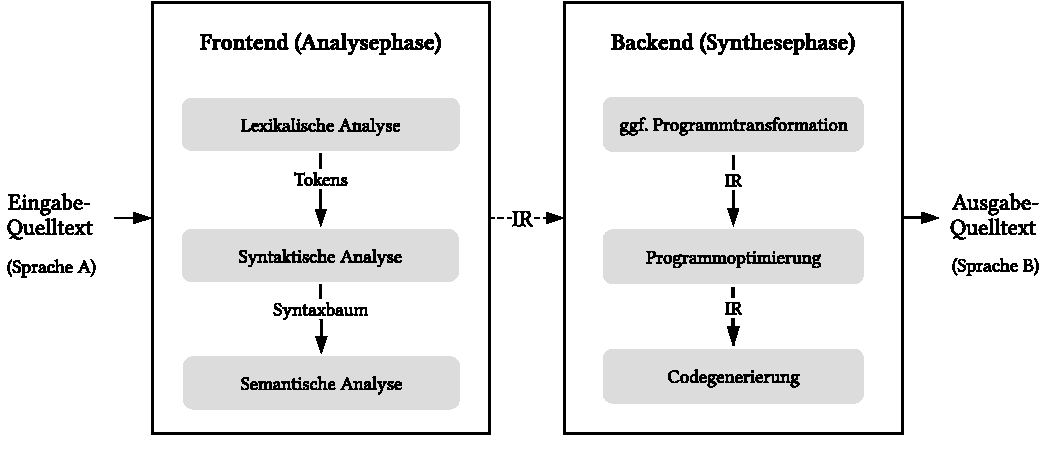
\includegraphics[width=\textwidth]{src/2_Grundlagen/fig/transpiler-architecture.pdf}
  \caption{Architektur eines typischen Transpilers nach~\autocite{EVGENIY:2016} und~\autocite[8]{TORCZON:2007}.}
	\label{fig:transpiler-architecture}
\end{figure}

Zunächst wird der Eingabequelltext innerhalb der Analysephase durch den Lexer oder Tokenizer Zeichen für Zeichen eingelesen, um diesen in lexikalisch bedeutungsvolle Zeichenketten, sogenannte \emph{Lexeme}, zu zerlegen~\autocite[43]{AHO:COMPILERS}. Daraufhin werden \emph{Tokens} gebildet, indem jedes dieser Wörter einer syntaktischen Klasse zugeordnet wird. Diese geben die Bedeutung eines Tokens an (zum Beispiel \code{3}~$\mapsto$~\code{INT(3)} oder \code{!=}~$\mapsto$~\code{NEQ})~\autocite[26]{TORCZON:2007}. Die Tokens entsprechen dabei den Terminalsymbolen der formalen Grammatik der Programmiersprache~\autocite[43]{AHO:COMPILERS}.

Im zweiten Schritt, der syntaktischen Analyse oder dem \emph{Parsen}, wird anschließend überprüft, ob die Tokenfolge eine Ableitung der kontextfreien Grammatik der Quellsprache darstellen, indem versucht wird, einen entsprechenden \emph{konkreten} Syntaxbaum aufzubauen~\autocite{SCHOEPP:COMPILER}. Ein Syntax- oder Ableitungsbaum ist ein Graph, der die syntaktische Struktur eines Programms gemäß der zugehörigen Grammatik hierarchisch modelliert. Abbildung~\ref{fig:ast} zeigt exemplarisch den \emph{abstrakten} Syntaxbaum (AST) einer simplen JavaScript-Funktion. Ein abstrakter Syntaxbaum ist eine kompaktere Form des konkreten Baums und zeigt lediglich \enquote{wesentliche Teile}~\autocite[21]{WALDMANN:PPS} davon. Falls der Ableitungsbaum nicht erstellt werden kann, so liegt ein Syntaxfehler im Quelltext vor.

\bigbreak
\begin{figure}[htb]
  {
    \begin{lstlisting}[numbers=none,aboveskip=0pt,belowskip=0pt]
    function square(x) {
      return x ** 2;
    }
    \end{lstlisting}
    \vspace{-0.5cm}
    \begin{center}
      \ttfamily
      \begin{forest}
        [FunctionDeclaration
          [Identifier, edge label={node[edge]{id}}
            [square, edge label={node[edge]{name}}]
          ]
          [Identifier{[]}, edge label={node[edge]{params}}
            [x, edge label={node[edge]{name}}]
          ]
          [BlockStatement, for tree = {s sep=1.3cm}, edge label={node[edge]{body}}
            [ReturnStatement, edge label={node[edge]{body}}
              [BinaryExpression, edge label={node[edge]{argument}}
                [Identifier, edge label={node[edge]{left}}
                  [x, tier=last, edge label={node[edge]{name}}]
                ]
                [**, tier=last, edge label={node[edge]{operator}}]
                [Literal, edge label={node[edge]{right}}
                  [2, tier=last, edge label={node[edge]{value}}]
                ]
              ]
            ]
          ]
        ]
      \end{forest}
    \end{center}
  }
  \caption{Abstrakter Syntaxbaum der obigen JavaScript-Funktion gemäß der Spezifikation \textit{ESTree}~\autocite{ESTREE_SPEC}.}
  \label{fig:ast}
\end{figure}

Danach prüft der Transpiler, ob ein gültiges Programm der Eingabesprache vorliegt, indem die statische Semantik analysiert wird~\autocite[8]{AHO:COMPILERS}. Hierunter fällt beispielsweise, dass Variablen in vielen Programmiersprachen vor deren Benutzung zunächst deklariert werden müssen. Um ein solches kontextuelles Programmverhalten zu untersuchen, können Attributgrammatiken verwendet werden~\autocite[161]{TORCZON:2007}. Während dieser Phase wird auch die Typkorrektheit überprüft, sofern ein statisches Typsystem vorliegt~\autocite{SCHOEPP:COMPILER}. Es ist hervorzuheben, dass nicht alle Transcompiler eine semantische Analyse durchführen, sondern manche unmittelbar zum nächsten Schritt übergehen.
Zuletzt wird durch das Frontend ein \emph{Zwischencode}\footnote{engl. \textit{intermediate representation} (IR).} des Programms erzeugt, der an das Backend übergeben wird. Ein Zwischencode ist im Allgemeinen eine von der Quellsprache und Zielarchitektur unabhängige Datenstruktur innerhalb von Compilern~\autocite[6]{TORCZON:2007}. Wie Abschnitt~\ref{sec:js-transpilers} zeigen wird, verwenden viele Transpiler im JavaScript-Umfeld den abstrakten Syntaxbaum als Zwischencode.

Der erste Schritt der darauffolgenden Synthesephase besteht darin, den Zwischencode gegebenenfalls zu transformieren, um gewünschte Programmeigenschaften herzustellen. Zum Beispiel könnte hier veraltete Syntax durch modernere Notationen ersetzt werden. Als nächstes wird das Programm sprachunabhängig optimiert, das heißt, die Laufzeit oder der Speicherplatzbedarf werden auf Basis einer Programmanalyse reduziert~\autocite[405]{TORCZON:2007}. Hierbei können eine Vielzahl unterschiedlicher Transformationen angewandt werden. Möglich ist zum Beispiel die Entfernung nicht erreichbarer Programmstücke (\textit{dead code elimination}) oder die Inline-Ersetzung von Konstanten und Schleifen~\autocites{TORCZON:2007}{SCHOEPP:COMPILER}. Auch hier gilt es zu betonen, dass nicht alle Transcompiler eine derartige Optimierungsphase besitzen.

Schließlich kann im letzten Schritt der endgültige Quelltext in der Zielsprache durch den modifizierten Zwischencode generiert werden~\autocite[505]{AHO:COMPILERS}. Die erzeugten Ausgabe kann dabei dem ursprünglichen Programm ähneln oder völlig andersartig aufgebaut sein, wenn beispielsweise die Namen aller Bezeichner im Quelltext gekürzt wurden, um ein kleineres Programm zu erzeugen (\textit{minification})~\autocite{FOWLER:TRANSPARENT}.

\subsection{Evaluation bestehender Werkzeuge zur Quelltext-Transformation}
\label{sec:js-transpilers}

Im Umfeld von JavaScript sind im Lauf der Jahre eine Vielzahl von Parsern, Codegeneratoren und Transpilern entstanden, welche die Entwicklung weiterer Software wie die des angestrebten Flow-Transcompilers stark vereinfachen können. Weil diese Werkzeuge bereits einen Großteil der benötigten Standardfunktionalität wie dem Einlesen und dem Generieren von Code bereit stellen, muss oftmals nur der Kern des Übersetzers, also im vorliegenden Fall die Transformation der Flow-Typen nach TypeScript, implementiert werden. Im Folgenden sollen einige der relevantesten aktuellen Werkzeuge bezüglich verschiedener Aspekte gegenüber gestellt werden, sodass daraufhin die Entscheidung getroffen werden kann, welcher der Ansätze als Grundlage für die Umsetzung des Transpilers herangezogen wird. Dabei wird nur frei verfügbare, quelloffene Software betrachtet.

Die Auswahl des Werkzeugs hängt entscheidend von der Erfüllung mehrerer technischer Anforderungen ab, die auf Basis der gegebenen Rahmenbedingungen innerhalb des Unternehmens Spreadshirt erarbeitet wurden und in Kapitel~\ref{chap:analysis} ausführlich dargelegt werden. Die erste Vorgabe ist die vollumfängliche Unterstützung aktueller JavaScript-Syntax gemäß der ECMAScript-Spezifikation 2019~\autocite{ECMASCRIPT:2019}. Weiterhin muss die Verarbeitung von \emph{vorläufiger} Syntax durch den Transpiler möglich sein. Darunter werden in dieser Arbeit Erweiterungen von JavaScript verstanden, die noch nicht endgültiger Bestandteil des ECMAScript-Standards sind. Dieser wird kontinuierlich durch das \textit{Technical Committee 39} (TC39)~\autocite{TC39_COMMITTEE} weiterentwickelt. Vorgeschlagene Spracherweiterungen durchlaufen dabei einen mehrstufigen Standardisierungsprozess, der letztlich in die Aufnahme in die Spezifikation münden kann~\autocite{TC39_PROCESS}. Derartige Syntax einlesen zu können, ist ebenfalls eine Anforderung, weil diese zum Teil bereits heute in den gegebenen Projekte von Spreadshirt eingesetzt werden\footnote{Dies setzt die Benutzung eines Transpilers wie Babel~\autocite{BABEL} voraus, der solche experimentelle Syntax vor der Auslieferung durch entsprechende Plugins in standardkonformes JavaScript transformiert.}. Damit die Übersetzung der Flow-Typen nach TypeScript möglich ist, muss ferner sowohl die Syntax von Flow, als auch von TypeScript vollständig unterstützt werden. Darüber hinaus muss sogenannte JSX-Syntax~\autocite{SOFTWARE:JSX} (\textit{JavaScript XML}) eingelesen werden können, weil die zu migrierenden Projekte auch diese Notation einsetzen. Die letzte Anforderung ist schließlich, dass auf Grundlage des transformierten Programms entsprechender TypeScript-Code generiert werden muss.

\begingroup
\setlength{\tabcolsep}{6pt} % reset to default
\begin{table}[tb]
  \footnotesize
  \begin{tabu} to \textwidth {@{}lllccccccrrX@{}}
    \midrule
    \libertineSB{Werkzeug} & \libertineSB{Typ} & \libertineSB{Format} & \libertineSB{Erw.} & \libertineSB{ES10} & \libertineSB{ES10+} & \libertineSB{Flow} & \libertineSB{TS} & \libertineSB{JSX} & \libertineSB{Aktivität} & \libertineSB{Sterne} \\
    \midrule
    Acorn     & P  &  ESTree  & \pie{2} & \pie{2} & \pie{1} & \pie{0} & \pie{0} & \pie{2} &   5 &  5.250 & {\autocite{ACORN}} \\ % 2012
    Astring   & G  &  ESTree  & \pie{2} & \pie{2} & \pie{1} & \pie{0} & \pie{0} & \pie{0} &  61 &    500 & {\autocite{ASTRING}} \\ % 2015
    Babel     & PG &  Babel   & \pie{2} & \pie{2} & \pie{2} & \pie{2} & \pie{2} & \pie{2} & 225 & 34.650 & {\autocite{BABEL}} \\ % 2014
    Escodegen & G  &  ESTree  & \pie{0} & \pie{0} & \pie{0} & \pie{0} & \pie{0} & \pie{0} &   2 &  1.900 & {\autocite{ESCODEGEN}} \\ % 2012
    Esprima   & P  &  ESTree  & \pie{0} & \pie{1} & \pie{0} & \pie{0} & \pie{0} & \pie{1} &  12 &  5.450 & {\autocite{ESPRIMA}} \\ % 2011
    Recast    & PG &  diverse & \pie{2} & \pie{2} & \pie{2} & \pie{2} & \pie{2} & \pie{2} &  43 &  2.700 & {\autocite{RECAST}} \\ % 2012
    \midrule
  \end{tabu}
  \caption*{
    \footnotesize
    \begin{minipage}[t]{.4\linewidth}
      {
        \renewcommand{\arraystretch}{1.1}
        \begin{tabular}{@{}ll@{}}
          P & Parser\\
          G & Codegenerator\\
          \pie{0} & keine Unterstützung\\
          \pie{1} & unvollständige Unterstützung\\
          \pie{2} & vollständige Unterstützung\\
        \end{tabular}
      }
    \end{minipage}
    \begin{minipage}[t]{.55\linewidth}
      {
        \renewcommand{\arraystretch}{1.1}
        \begin{tabular}{@{}ll@{}}
          Erw. & Erweiterbarkeit\\
          ES10 & ECMAScript 2019\\
          ES10+ & vorgeschlagene JavaScript-Erweiterungen\\
          TS & TypeScript\\
          Sterne & Anzahl der Sterne auf GitHub\\
        \end{tabular}
      }
    \end{minipage}

    \medbreak
    \begin{justify}
      Aktivität: Entspricht der Summe der Zahl von \emph{Merge Requests}, neuer bzw. geschlossener Fehlerberichte, veröffentlichter Git-Commits auf dem Hauptzweig und der Anzahl beteiligter Autoren innerhalb eines Monats auf der Plattform GitHub~\autocite{GITHUB} (Stand Oktober 2019).
    \end{justify}
  }
  \caption{Vergleich verschiedener Werkzeuge zur Transpilierung von JavaScript"=Quelltexten.}
  \label{tab:transpilers}
\end{table}
\endgroup


Die Eigenschaften der in Betracht kommenden Werkzeuge werden in Tabelle~\ref{tab:transpilers} aufgelistet. Dabei werden verschiedene Parser (\textit{Acorn}, \textit{Esprima}), Codegeneratoren (\textit{Astring}, \textit{Escodegen}) und ganze Transpiler (\textit{Babel}, \textit{Recast}) für JavaScript betrachtet. Jedes der Werkzeuge benutzt intern den abstrakten Syntaxbaum der Eingabe als Zwischencode. Da außer Babel alle Alternativen die Spezifikation \textit{ESTree} für den Aufbau des abstrakten Syntaxbaums verwenden, können diese Parser und Codegeneratoren prinzipiell beliebig kombiniert werden, um einen Transcompiler zusammenzusetzen. Der ESTree-Standard wird von Mitgliedern verschiedener Projekte im Umfeld der statischen Analyse von JavaScript stetig weiterentwickelt und spezifiziert den Aufbau abstrakter Syntaxbäume von ECMAScript-Programmen~\autocite{ESTREE_SPEC}. Weil aber weder Astring, noch Escodegen TypeScript als Ausgabesprache unterstützen, kann dieser Ansatz nicht verfolgt werden, um die gegebene Problemstellung zu lösen.

Nach Kenntnisstand des Autors existieren außer Babel und Recast keine weiteren Werkzeuge, die einen Codegenerator bereitstellen, der TypeScript auf Grundlage von JavaScript-Syntaxbäumen erzeugen kann. Auch sind diese Projekte die einzigen der betrachteten, die aktuelle und vorläufige JavaScript-Syntax sowie Flow, TypeScript und JSX vollständig verarbeiten können. Jedoch wird dies in Recast nur bei Verwendung des Parsers von Babel~\autocite{BABEL:PARSER} erzielt. Recast setzt standardmäßig Esprima als Parser ein, aber es können auch anderer Parser wie Babel verwendet werden, um nicht standardkonforme Syntax-Erweiterungen von JavaScript einzulesen. Ein interessantes Merkmal von Recast ist, dass hier die Formatierung der Ausgabe konsistent beibehalten wird, indem die abstrakten Syntaxbäume der Ein- und Ausgabe verglichen werden, sodass daraufhin nur der Code der geänderten Teilbäume neu generiert wird~\autocite{RECAST}. Dieser Ansatz wirkt zunächst aussichtsreich, weil so eine originalgetreue Formatierung der Ausgabe des angestrebten Transpilers erreicht werden könnte. Jedoch hat sich experimentell gezeigt, dass die Formatierung der geänderten und damit neu generierten Programmteile, anders als von Recast behauptet, zum Teil vom ursprünglichen Code abweicht. Der Programmierstil unveränderter Abschnitte wird tatsächlich präzise beibehalten. Auch wurde festgestellt, dass Kommentare innerhalb der modifizierten Ausdrücke komplett verloren gehen, was für die Erzielung einer korrekten Übersetzung inakzeptabel ist.

Weil Babel im Vergleich zu Recast deutlich verbreiteter ist und aktiver entwickelt wird, kann Babel als die ausgereiftere Software betrachtet werden (vgl. Tabelle). Darüber hinaus bietet Babel eine gute Erweiterbarkeit durch ein Plugin-System~\autocite{BABEL:HANDBOOK} und besitzt eine umfangreiche Dokumentation~\autocite{BABEL:DOCS}. Aufgrund dieser Vorteile und Alleinstellungsmerkmale wird Babel als Grundlage für die Implementierung gewählt.

\subsection{Babel}
\label{sec:babel}

\subsubsection{Funktionsweise}

Zur Erleichterung des Verständnisses der Ausführung der Umsetzung des Flow-Transpilers in Kapitel \ref{chap:implementation} soll zunächst die grundsätzliche Funktionsweise von Babel umrissen werden. Die Ausführung von Babel gliedert sich in folgende drei Phasen~\autocite{BABEL:HANDBOOK}. Diese sind in weiten Teilen analog zu dem beschriebenen Aufbau eines typischen Transcompilers.

\begin{enumerate}
  \item {\libertineSB{Parsen des Eingabecodes}}\\*
    Zunächst wird der ursprüngliche Quelltext in zwei Schritten eingelesen, um den abstrakten Syntaxbaum des Programms zu erzeugen: Als Erstes wird der Code während der lexikalischen Analyse mittels des Lexers in Tokens zerlegt. Anschließend werden diese in der syntaktischen Analyse zu einer Datenstruktur umgeformt, die den zugehörigen abstrakten Syntaxbaum repräsentiert. Jedem Knoten des Baums wird dabei einen eindeutiger Tokentyp zugewiesen, der die syntaktische Bedeutung widerspiegelt.
    \bigbreak
  \item {\libertineSB{Transformation des Programms}}\\*
    Während der zweiten Phase wird daraufhin die Kernfunktionalität von Babel, die Programmtransformation umgesetzt: Dabei wird der abstrakte Syntaxbaum durch das \emph{Besucher}"=Entwurfsmuster\footnote{Das Besucher-Entwurfsmustern (engl. \textit{visitor pattern}) gehört zu den 23 Entwurfsmustern, die im Standardwerk \citetitle{GAMMA:1994} der \enquote{\textit{Gang of Four}} (E. Gamma, R. Helm, R. Johnson und J. Vlissides) beschrieben werden~\autocite[306\psqq]{GAMMA:1994}.} rekursiv traversiert und die Knoten des Baums sukzessive modifiziert, gelöscht bzw. neu erstellte Elemente eingefügt. Das Entwurfsmuster beschreibt, wie ein Algorithmus auf einer komplexen Objektdatenstruktur, unabhängig von der konkreten Implementierung der zugrunde liegenden Klassen, ausgeführt werden kann~\autocite[634\psq]{FREEMAN:2004}. Im vorliegenden Fall ermöglicht die Anwendung die individuelle Adressierung einer bestimmten Untermenge der Knoten des Syntaxbaums, sodass dort die gewünschte Transformation des Programms durchgeführt werden kann.
    \bigbreak
  \item {\libertineSB{Generierung des Ausgabequelltexts}}\\*
    Schließlich kann der Ausgabecode generiert werden: Hierbei werden alle Knoten des abstrakten Syntaxbaums durch Anwendung einer Tiefensuche durchlaufen und eine Zeichenkette aufgebaut, die den endgültigen, modifizierten Quelltext darstellt.
\end{enumerate}

\subsubsection{Babel-Plugins}
\label{sec:babel-plugins}

Da die entscheidende Phase der Transpilierung, die Programmtransformation, bei Babel durch Plugins erzielt wird, sollen diese genauer betrachtet werden. Plugins sind die elementaren Bausteine, die eine flexible Erweiterung von Babel ermöglichen. Selbst der Kern des Transcompilers ist aus einer Vielzahl von Standard-Plugins zusammen gesetzt, die in ihrer Gesamtheit die Funktionalität des Systems abbilden~\autocite{BABEL}. Dies verdeutlicht die tiefgreifende Modularität der Architektur von Babel.

Ein Babel-Plugin ist eine JavaScript"=Funktion, welche gemäß der vorgegebenen Schnittstellen ein Objekt mit verschiedenen Attributen zurückliefern muss. Mindestens anzugeben ist dabei lediglich die Abbildung der gewünschten Knotentypen des abstrakten Syntaxbaums auf Besucherfunktionen~\autocite{BABEL:HANDBOOK}. Deren Implementierung setzt die angestrebte Quelltext"=Transformation um. Es ist in der Praxis gängig mehrere Plugins einzusetzen, sodass ein Knoten während der Verarbeitung durch Babel mehrere, unabhängige Transformationen durchlaufen kann. Hierdurch kann die erwünschte Transpilierung von JavaScript-Quelltexten flexibel durch Kombination vieler, kleiner Bausteine realisiert werden. Auch möglich ist die Angabe einer hierarchischen Abhängigkeitsstruktur, sodass dass die Verwendung eines Plugins zur impliziten Aktivierung weiterer Plugins führt.

Der konkrete Aufbau von Babel-Plugins soll durch ein Minimalbeispiel gezeigt werden. Quelltext~\ref{code:babel-plugin-definition} zeigt den Code eines simplen aber vollständigen Plugins, welches lediglich den Namen aller Bezeichner (\code{Identifier}) eines JavaScript-Programms in Großbuchstaben setzt. Hierfür wird eine gleichnamige Besucherfunktion für den Knotentyp \code{Identifier} definiert (Zeile~5). Diese erhält den \emph{Pfad} der so adressierten Identifier-Knoten als Argument und kann diesen wie gewünscht transformieren. Der Pfad eines AST-Knotens ist ein Objekt, das die Beziehung des Knotens zu seinen Elternelementen modelliert und diesen um Metainformationen anreichert~\autocite{BABEL:HANDBOOK}. Es enthält eine Vielzahl von Methoden mittels derer der Pfad und der Syntaxbaum manipuliert werden kann.

\begin{lstlisting}[
  % float,
  % floatplacement=H,
  label={code:babel-plugin-definition},
  caption={[Minimalbeispiel eines Babel-Plugins]Minimalbeispiel eines Babel-Plugins: Die Namen aller Bezeichner (\code{Identifier}) werden in Großbuchstaben umgewandelt.}
]
// var foo => var FOO
module.exports = function() {
  return {
    visitor: {
      Identifier(path) {
        path.node.name = path.node.name.toUpperCase();
      }
    }
  };
};
\end{lstlisting}

Alle Knotentypen des abstrakten Syntaxbaums von Babel werden einerseits in der Spezifikation des Parsers~\autocite{BABEL:PARSER_SPEC,BABEL:PARSER}, andererseits in der Dokumentation der Bibliothek \code{@babel/types}~\autocite{BABEL:TYPES} beschrieben.
Der Aufbau des von Babel eingesetzten abstrakten Syntaxbaums liegt in einem eigenen Format vor, das auf dem ESTree-Standard~\autocite{ESTREE_SPEC} basiert. Mit der sechsten Version von Babel wurde entschieden, von der ESTree-Spezifikation abzuweichen, damit auch vorläufige JavaScript-Erweiterungen unterstützen werden können~\autocite{BABEL:STATE_OF_BABEL}.

Im weitere Verlauf wird das Hauptaugenmerk der Untersuchung auf die zweite Phase der Transpilierung durch Babel gelegt, da hier die vorliegende Problemstellung, die Transformation der Flow-Typannotationen nach TypeScript, umgesetzt wird. Das Parsen des Eingabquelltexts und das Generieren der Ausgabe kann durch Verwendung der gegebenen Bibliotheksfunktionen von Babel simpel realisiert werden und bedarf keiner genaueren Betrachtung.
